% TG-LiteNet -- CSD361 final report (IEEE conference format, 8 pages).
% Build:  python scripts/make_paper.py   (tables, figures and numbers.tex from results/)   then   pdflatex main (twice).
\documentclass[conference]{IEEEtran}
\IEEEoverridecommandlockouts
\setlength{\textfloatsep}{5pt plus 2pt minus 2pt}\setlength{\floatsep}{6pt plus 2pt minus 2pt}\setlength{\intextsep}{6pt plus 2pt minus 2pt}
\setlength{\abovecaptionskip}{2pt}\setlength{\belowcaptionskip}{0pt}
\usepackage{cite}
\usepackage{amsmath,amssymb,amsfonts}
\usepackage{algorithmic}
\usepackage{algorithm}
\usepackage{graphicx}
\usepackage{textcomp}
\usepackage{xcolor}
\usepackage{booktabs}
\usepackage{multirow}
\usepackage{adjustbox}
\usepackage{url}
\usepackage{tikz}
\usetikzlibrary{arrows.meta,positioning,shapes.geometric,fit,backgrounds,calc}
% auto-generated by scripts/make_paper.py - do not edit
\newcommand{\uDiceRawA}{0.759}
\newcommand{\uDiceTunedA}{0.762}
\newcommand{\uDiceCleanA}{0.759}
\newcommand{\uClRawA}{0.836}
\newcommand{\uBettiRawA}{72.8}
\newcommand{\uBettiCleanA}{4.5}
\newcommand{\gapRawA}{0.066}
\newcommand{\gapTunedA}{0.061}
\newcommand{\driveRawA}{0.825}
\newcommand{\cpuA}{936}
\newcommand{\parA}{31.04}
\newcommand{\uDiceRawB}{0.758}
\newcommand{\uDiceTunedB}{0.775}
\newcommand{\uDiceCleanB}{0.759}
\newcommand{\uClRawB}{0.842}
\newcommand{\uBettiRawB}{33.9}
\newcommand{\uBettiCleanB}{4.4}
\newcommand{\gapRawB}{0.063}
\newcommand{\gapTunedB}{0.043}
\newcommand{\driveRawB}{0.821}
\newcommand{\cpuB}{989}
\newcommand{\parB}{31.04}
\newcommand{\uDiceRawC}{0.761}
\newcommand{\uDiceTunedC}{0.789}
\newcommand{\uDiceCleanC}{0.763}
\newcommand{\uClRawC}{0.846}
\newcommand{\uBettiRawC}{35.5}
\newcommand{\uBettiCleanC}{4.6}
\newcommand{\gapRawC}{0.064}
\newcommand{\gapTunedC}{0.035}
\newcommand{\driveRawC}{0.824}
\newcommand{\cpuC}{1003}
\newcommand{\parC}{31.04}
\newcommand{\uDiceRawD}{0.749}
\newcommand{\uDiceTunedD}{0.780}
\newcommand{\uDiceCleanD}{0.751}
\newcommand{\uClRawD}{0.835}
\newcommand{\uBettiRawD}{40.5}
\newcommand{\uBettiCleanD}{4.6}
\newcommand{\gapRawD}{0.070}
\newcommand{\gapTunedD}{0.039}
\newcommand{\driveRawD}{0.819}
\newcommand{\cpuD}{31}
\newcommand{\parD}{0.49}
\newcommand{\uDiceRawE}{0.751}
\newcommand{\uDiceTunedE}{0.780}
\newcommand{\uDiceCleanE}{0.753}
\newcommand{\uClRawE}{0.836}
\newcommand{\uBettiRawE}{39.2}
\newcommand{\uBettiCleanE}{4.4}
\newcommand{\gapRawE}{0.067}
\newcommand{\gapTunedE}{0.037}
\newcommand{\driveRawE}{0.817}
\newcommand{\cpuE}{30}
\newcommand{\parE}{0.49}
\newcommand{\uDiceRawEmc}{0.752}
\newcommand{\uDiceTunedEmc}{0.778}
\newcommand{\cpuEmc}{600}
\newcommand{\gpuA}{27.8}
\newcommand{\gpuE}{3.3}
\newcommand{\gflopsA}{385}
\newcommand{\gflopsE}{6.05}
\newcommand{\fivesRawX}{0.849}
\newcommand{\uDiceRawX}{0.774}
\newcommand{\uDiceTunedX}{0.785}
\newcommand{\uBettiRawX}{91.1}
\newcommand{\uDiceTunedWarm}{0.791}
\newcommand{\uDiceRawWarm}{0.761}
\newcommand{\cpuKeight}{38}
\newcommand{\parKeight}{0.49}
\newcommand{\cpuKsixteen}{86}
\newcommand{\parKsixteen}{1.94}
\newcommand{\cpuKlite}{109}
\newcommand{\parKlite}{0.21}
\newcommand{\cpuKhyb}{89}
\newcommand{\parKhyb}{0.26}
\newcommand{\HTuned}{0.768}
\newcommand{\HSel}{0.779}
\newcommand{\HRaw}{0.733}
\newcommand{\HCl}{0.820}
\newcommand{\HBetti}{32.1}
\newcommand{\HDrive}{0.810}
\newcommand{\HFives}{0.810}
\newcommand{\HParams}{66K}
\newcommand{\HGflops}{2.73}
\newcommand{\HCpu}{24.7}
\newcommand{\HHrf}{0.729}
\newcommand{\HStare}{0.810}
\newcommand{\HChase}{0.765}
\newcommand{\RlTuned}{0.775}
\newcommand{\RlSel}{0.785}
\newcommand{\RlRaw}{0.745}
\newcommand{\RlCl}{0.826}
\newcommand{\RlBetti}{29.0}
\newcommand{\RlDrive}{0.814}
\newcommand{\RlFives}{0.822}
\newcommand{\RlParams}{212K}
\newcommand{\RlGflops}{5.53}
\newcommand{\RlCpu}{106.7}
\newcommand{\RlHrf}{0.736}
\newcommand{\RlStare}{0.812}
\newcommand{\RlChase}{0.777}
\newcommand{\RuTuned}{0.775}
\newcommand{\RuSel}{0.785}
\newcommand{\RuRaw}{0.739}
\newcommand{\RuCl}{0.826}
\newcommand{\RuBetti}{31.8}
\newcommand{\RuDrive}{0.812}
\newcommand{\RuFives}{0.822}
\newcommand{\RuParams}{486K}
\newcommand{\RuGflops}{6.05}
\newcommand{\RuCpu}{55.0}
\newcommand{\RuHrf}{0.736}
\newcommand{\RuStare}{0.812}
\newcommand{\RuChase}{0.775}
\newcommand{\ENSHTuned}{0.773}
\newcommand{\ENSHSel}{0.785}
\newcommand{\ENSHRaw}{0.741}
\newcommand{\ENSHCl}{0.827}
\newcommand{\ENSHBetti}{26.5}
\newcommand{\ENSHDrive}{0.814}
\newcommand{\ENSHFives}{0.828}
\newcommand{\ENSHParams}{66K}
\newcommand{\ENSHGflops}{2.73}
\newcommand{\ENSHCpu}{24.7}
\newcommand{\ENSHHrf}{0.730}
\newcommand{\ENSHStare}{0.817}
\newcommand{\ENSHChase}{0.772}
\newcommand{\EvTuned}{0.780}
\newcommand{\EvSel}{0.789}
\newcommand{\EvRaw}{0.751}
\newcommand{\EvCl}{0.825}
\newcommand{\EvBetti}{39.2}
\newcommand{\EvDrive}{0.817}
\newcommand{\EvFives}{0.847}
\newcommand{\EvParams}{486K}
\newcommand{\EvGflops}{6.05}
\newcommand{\EvCpu}{30.0}
\newcommand{\EvHrf}{0.733}
\newcommand{\EvStare}{0.819}
\newcommand{\EvChase}{0.787}
\newcommand{\CvTuned}{0.789}
\newcommand{\CvSel}{0.751}
\newcommand{\CvRaw}{0.761}
\newcommand{\CvCl}{0.836}
\newcommand{\CvBetti}{35.5}
\newcommand{\CvDrive}{0.824}
\newcommand{\CvFives}{0.842}
\newcommand{\CvParams}{31036K}
\newcommand{\CvGflops}{384.74}
\newcommand{\CvCpu}{1003.4}
\newcommand{\CvHrf}{0.749}
\newcommand{\CvStare}{0.828}
\newcommand{\CvChase}{0.789}
\newcommand{\ENSDTuned}{0.783}
\newcommand{\ENSDSel}{0.792}
\newcommand{\ENSDRaw}{0.754}
\newcommand{\ENSDCl}{0.829}
\newcommand{\ENSDBetti}{31.4}
\newcommand{\ENSDDrive}{0.820}
\newcommand{\ENSDFives}{0.856}
\newcommand{\ENSDParams}{2432K}
\newcommand{\ENSDGflops}{30.24}
\newcommand{\ENSDCpu}{154.4}
\newcommand{\ENSDHrf}{0.738}
\newcommand{\ENSDStare}{0.823}
\newcommand{\ENSDChase}{0.788}
\newcommand{\ZvtwoTuned}{0.777}
\newcommand{\ZvtwoSel}{0.782}
\newcommand{\ZvtwoRaw}{0.750}
\newcommand{\ZvtwoCl}{0.819}
\newcommand{\ZvtwoBetti}{41.5}
\newcommand{\ZvtwoDrive}{0.815}
\newcommand{\ZvtwoFives}{0.830}
\newcommand{\ZvtwoParams}{66K}
\newcommand{\ZvtwoGflops}{2.73}
\newcommand{\ZvtwoCpu}{24.2}
\newcommand{\ZvtwoHrf}{0.730}
\newcommand{\ZvtwoStare}{0.816}
\newcommand{\ZvtwoChase}{0.783}
\newcommand{\thrA}{0.52}
\newcommand{\precRawA}{0.665}
\newcommand{\sensRawA}{0.895}
\newcommand{\precTunedA}{0.679}
\newcommand{\sensTunedA}{0.879}
\newcommand{\thrB}{0.59}
\newcommand{\precRawB}{0.663}
\newcommand{\sensRawB}{0.895}
\newcommand{\precTunedB}{0.707}
\newcommand{\sensTunedB}{0.867}
\newcommand{\thrC}{0.65}
\newcommand{\precRawC}{0.655}
\newcommand{\sensRawC}{0.915}
\newcommand{\precTunedC}{0.725}
\newcommand{\sensTunedC}{0.873}
\newcommand{\thrD}{0.66}
\newcommand{\precRawD}{0.641}
\newcommand{\sensRawD}{0.908}
\newcommand{\precTunedD}{0.715}
\newcommand{\sensTunedD}{0.863}
\newcommand{\thrE}{0.64}
\newcommand{\precRawE}{0.645}
\newcommand{\sensRawE}{0.906}
\newcommand{\precTunedE}{0.717}
\newcommand{\sensTunedE}{0.861}
\newcommand{\dABDice}{\ensuremath{-}0.0009}
\newcommand{\ciABDice}{0.0114}
\newcommand{\pABDice}{1.000}
\newcommand{\dABCl}{+0.0057}
\newcommand{\ciABCl}{0.0098}
\newcommand{\pABCl}{1.000}
\newcommand{\dABBetti}{\ensuremath{-}38.9}
\newcommand{\ciABBetti}{17.3}
\newcommand{\pABBetti}{0.069}
\newcommand{\dABGap}{\ensuremath{-}0.0026}
\newcommand{\ciABGap}{0.0152}
\newcommand{\pABGap}{1.000}
\newcommand{\dBCDice}{+0.0027}
\newcommand{\ciBCDice}{0.0085}
\newcommand{\pBCDice}{1.000}
\newcommand{\dBCCl}{+0.0039}
\newcommand{\ciBCCl}{0.0107}
\newcommand{\pBCCl}{1.000}
\newcommand{\dBCBetti}{+1.6}
\newcommand{\ciBCBetti}{4.4}
\newcommand{\pBCBetti}{1.000}
\newcommand{\dBCGap}{+0.0002}
\newcommand{\ciBCGap}{0.0079}
\newcommand{\pBCGap}{1.000}
\newcommand{\dCDDice}{\ensuremath{-}0.0114}
\newcommand{\ciCDDice}{0.0062}
\newcommand{\pCDDice}{0.132}
\newcommand{\dCDCl}{\ensuremath{-}0.0105}
\newcommand{\ciCDCl}{0.0027}
\newcommand{\pCDCl}{0.009}
\newcommand{\dCDBetti}{+5.0}
\newcommand{\ciCDBetti}{6.4}
\newcommand{\pCDBetti}{1.000}
\newcommand{\dCDGap}{+0.0062}
\newcommand{\ciCDGap}{0.0054}
\newcommand{\pCDGap}{0.534}
\newcommand{\dAEmcBetti}{\ensuremath{-}32.9}
\newcommand{\ciAEmcBetti}{10.9}
\newcommand{\pAEmcBetti}{0.024}
\newcommand{\dAEmcDice}{\ensuremath{-}0.0070}
\newcommand{\ciAEmcDice}{0.0059}
\newcommand{\dAEmcDiceTuned}{+0.0162}
\newcommand{\dABDiceTuned}{+0.0134}
\newcommand{\dBCDiceTuned}{+0.0140}
\newcommand{\dBCGapTuned}{\ensuremath{-}0.0083}
\newcommand{\dMcDice}{+0.0010}
\newcommand{\dMcDiceCi}{0.0005}
\newcommand{\dAXDice}{+0.0148}
\newcommand{\ciAXDice}{0.0052}
\newcommand{\dAXCl}{+0.0022}
\newcommand{\ciAXCl}{0.0055}
\newcommand{\dAXBetti}{+15.3}
\newcommand{\ciAXBetti}{33.9}
\newcommand{\dXCDice}{\ensuremath{-}0.0144}
\newcommand{\ciXCDice}{0.0203}
\newcommand{\dXCCl}{+0.0063}
\newcommand{\ciXCCl}{0.0050}
\newcommand{\dXCBetti}{\ensuremath{-}55.3}
\newcommand{\ciXCBetti}{37.0}
\newcommand{\nTrainVtwo}{76}
\newcommand{\nSeedsMain}{5}
\newcommand{\nTrainVtwoOne}{38}
\newcommand{\nTrainAll}{114}
\newcommand{\budgetIters}{10000}
\newcommand{\compactParams}{486}
\newcommand{\liteParams}{212}
\newcommand{\hParamsExact}{66\,125}
\newcommand{\hParamsK}{66}
\newcommand{\ratioParams}{469}
\newcommand{\ratioParamsE}{64}
\newcommand{\valRl}{0.8140}
\newcommand{\valH}{0.8085}
\newcommand{\valGap}{0.0055}
\newcommand{\nTwoH}{+0.0114}
\newcommand{\nTwoHci}{0.0005}
\newcommand{\nTwoHrf}{+0.034}
\newcommand{\nTwoFives}{\ensuremath{-}0.061}
\newcommand{\nTwoCv}{\ensuremath{-}0.0383}
\newcommand{\nTwoEv}{+0.0095}
\newcommand{\nTwoRl}{+0.0094}
\newcommand{\nTwoRu}{+0.0102}
\newcommand{\aNthreeDice}{\ensuremath{-}0.0051}
\newcommand{\aNthreeDiceci}{0.0148}
\newcommand{\aNthreeDicev}{not clear}
\newcommand{\aNthreeCl}{+0.0019}
\newcommand{\aNthreeClci}{0.0073}
\newcommand{\aNthreeClv}{not clear}
\newcommand{\aNthreeBetti}{\ensuremath{-}11.4963}
\newcommand{\aNthreeBettici}{15.7837}
\newcommand{\aNthreeBettiv}{not clear}
\newcommand{\aNfourDice}{\ensuremath{-}0.0091}
\newcommand{\aNfourDiceci}{0.0045}
\newcommand{\aNfourDicev}{clear}
\newcommand{\aNfourCl}{+0.0011}
\newcommand{\aNfourClci}{0.0105}
\newcommand{\aNfourClv}{not clear}
\newcommand{\aNfourBetti}{\ensuremath{-}3.9476}
\newcommand{\aNfourBettici}{20.0068}
\newcommand{\aNfourBettiv}{not clear}
\newcommand{\aAugDice}{\ensuremath{-}0.0094}
\newcommand{\aAugDiceci}{0.0267}
\newcommand{\aAugDicev}{not clear}
\newcommand{\aAugCl}{+0.0053}
\newcommand{\aAugClci}{0.0108}
\newcommand{\aAugClv}{not clear}
\newcommand{\aAugBetti}{+3.2969}
\newcommand{\aAugBettici}{19.8757}
\newcommand{\aAugBettiv}{not clear}
\newcommand{\aAllDice}{\ensuremath{-}0.0081}
\newcommand{\aAllDiceci}{0.0188}
\newcommand{\aAllDicev}{not clear}
\newcommand{\aAllCl}{+0.0015}
\newcommand{\aAllClci}{0.0143}
\newcommand{\aAllClv}{not clear}
\newcommand{\aAllBetti}{\ensuremath{-}9.2167}
\newcommand{\aAllBettici}{16.5123}
\newcommand{\aAllBettiv}{not clear}
\newcommand{\aKdDice}{\ensuremath{-}0.0033}
\newcommand{\aKdDiceci}{0.0044}
\newcommand{\aKdDicev}{not clear}
\newcommand{\aKdCl}{+0.0068}
\newcommand{\aKdClci}{0.0114}
\newcommand{\aKdClv}{not clear}
\newcommand{\aKdBetti}{\ensuremath{-}9.1538}
\newcommand{\aKdBettici}{12.5467}
\newcommand{\aKdBettiv}{not clear}
\newcommand{\nOneEmc}{+0.1073}
\newcommand{\nOneEmcci}{0.0625}
\newcommand{\nOneH}{\ensuremath{-}0.1374}
\newcommand{\nOneHci}{0.1275}
\newcommand{\nOneEd}{+0.0698}
\newcommand{\nOneEdci}{0.1767}
\newcommand{\nOneVsMc}{+0.1547}
\newcommand{\nOneVsMcci}{0.1095}
\newcommand{\rhoHEnt}{0.22}
\newcommand{\rhoHFrag}{0.08}
\newcommand{\rhoHEnd}{0.22}
\newcommand{\rhoHSmall}{0.16}
\newcommand{\rhoEdEnt}{0.04}
\newcommand{\rhoEdFrag}{0.11}
\newcommand{\rhoEdEnd}{0.18}
\newcommand{\rhoEdSmall}{0.20}
\newcommand{\rhoCEnt}{0.07}
\newcommand{\rhoCFrag}{0.22}
\newcommand{\rhoCEnd}{0.22}
\newcommand{\rhoCSmall}{0.32}
\newcommand{\rhoPxMin}{0.34}
\newcommand{\rhoPxMax}{0.34}
\newcommand{\rhoPxEmc}{0.34}
\newcommand{\rhoImgEmc}{\ensuremath{-}0.08}
\newcommand{\rhoImgHrfEmc}{\ensuremath{-}0.12}
\newcommand{\rhoImgHrfE}{\ensuremath{-}0.40}
\newcommand{\pxErrFull}{5.9}
\newcommand{\pxErrNinety}{2.4}
\newcommand{\eceE}{0.046}
\newcommand{\eceTsE}{0.053}
\newcommand{\hFpMs}{16.3}
\newcommand{\hIntMs}{24.8}
\newcommand{\hFpKb}{266}
\newcommand{\hIntKb}{109}
\newcommand{\scaleOneFiveHrf}{92}
\newcommand{\scaleOneHrf}{8}
\newcommand{\scaleOneFiveFives}{0}
\newcommand{\scaleOneFives}{90}
\newcommand{\scaleOneFiveStare}{0}
\newcommand{\scaleOneStare}{100}
\newcommand{\scaleOneFiveChase}{0}
\newcommand{\scaleOneChase}{100}
\newcommand{\scaleOneFiveDrive}{0}
\newcommand{\scaleOneDrive}{100}

\newcommand{\cl}{\mathrm{clDice}}
\newcommand{\safefig}[2]{\IfFileExists{figures/#2.pdf}{\includegraphics[width=#1]{figures/#2.pdf}}{\fbox{figure #2 missing}}}
\renewcommand{\IEEEkeywordsname}{Keywords}
\pdfinfo{/Title (Compact Topology-Aware Retinal Vessel Segmentation Under Dataset Shift: A Pre-Registered Study of TG-LiteNet) /Author (Abhiraj Agarwal, Tanish Shitanshu, Shashwat Rajan) /Subject (CSD361 Introduction to Machine Learning, Final Project Report, Group 22)}
\begin{document}

\title{Compact Topology-Aware Retinal Vessel Segmentation Under Dataset Shift: A Pre-Registered Study of TG-LiteNet with Test-Time Scale Selection}

\author{\begin{tabular}[t]{ccc}
Abhiraj Agarwal & Shashwat Rajan & Tanish Shitanshu\\
\normalsize Roll No.\ 2510110002 & \normalsize Roll No.\ 2510111019 & \normalsize Roll No.\ 2510110008
\end{tabular}\\[0.5em]
\normalsize CSD361 -- Introduction to Machine Learning, Final Project Report (Group 22)\\
\normalsize Department of Computer Science and Engineering, Shiv Nadar Institution of Eminence, Delhi NCR, India}
\maketitle

\begin{abstract}
Retinal vessel segmenters intended for screening must keep thin vessels connected, generalise to cameras they were not trained on, and run on modest hardware, but these requirements are rarely evaluated together. We study them for TG-LiteNet, a compact U-Net trained on 15 DRIVE images only and tested without adaptation on STARE, CHASE\_DB1, HRF and FIVES. Every rule, selection criterion and statistical test was written down and hashed before any target image was evaluated. Study v2 (\nTrainVtwo\ trainings, five seeds per stage) ablates a soft-clDice topology loss, robustness augmentation, a compact backbone and uncertainty estimates; v2.1 (\nTrainVtwoOne\ trainings) shrinks the model to \hParamsK\,K parameters and tests four topology-based ideas. The topology loss lowers the raw unseen Betti-0 error from \uBettiRawA\ to \uBettiRawB, but deleting small fragments brings every model to about 4.5, so raw fragment counts are not a reliable measure of connectivity. With a threshold tuned on DRIVE validation images the stages reach \uDiceTunedA--\uDiceTunedC\ unseen Dice, so the Dice cost of topology supervision at threshold 0.5 is largely calibration. A 486K compact U-Net is 31$\times$ faster on CPU than the 31M U-Net (\uDiceTunedE\ against \uDiceTunedC\ Dice), and depthwise convolutions were slower than plain ones. The \hParamsK K model ($\ratioParams\times$ smaller than the U-Net, \HCpu\,ms per image, \hIntKb\,KB as INT8) reaches \HTuned\ unseen Dice, and \HSel\ with a label-free calibre-guided test-time scale rule (gain \nTwoH, clear; HRF \nTwoHrf, FIVES \nTwoFives). Of the four ideas, test-time scale selection is clearly supported, secondary connectivity scores give a promising reliability lead, and distillation and skeleton consistency show no clear gain at this scale. Published lightweight models score 0.03--0.04 higher under different protocols.
\end{abstract}

\begin{IEEEkeywords}
retinal vessel segmentation, topology-aware loss, domain generalization, lightweight networks, test-time scale selection, pre-registration
\end{IEEEkeywords}

% =============================================================================== I
\section{Introduction}
Segmenting the retinal vasculature from fundus photographs underlies the measurement of vessel calibre, tortuosity and branching used in screening for diabetic retinopathy, glaucoma and hypertensive disease~\cite{liu2025review}. Since U-Net~\cite{ronneberger2015}, networks trained on small public datasets such as DRIVE~\cite{staal2004}, STARE~\cite{hoover2000}, CHASE\_DB1~\cite{fraz2012} and HRF~\cite{budai2013} have reached high overlap scores. Overlap hides a different failure: a vessel severed by one pixel barely changes the Dice coefficient yet breaks the connectivity on which downstream biomarkers depend~\cite{shit2021,shi2024,kirchhoff2024}.

\textbf{Motivation.} A model for a low-resource screening programme must satisfy three requirements simultaneously: (i) preserve vessel \emph{topology}; (ii) tolerate camera and annotation \emph{shift} without labelled data from the new site~\cite{galdran2022,fadugba2024}; and (iii) be small and fast enough for commodity hardware~\cite{zeng2025,sobhan2026}. Each has been studied separately, usually on a different evaluation protocol, which makes the trade-offs between them impossible to read.

\textbf{Problem statement and objectives.} Given a model trained on one dataset only, we ask how much a topology loss, robustness augmentation, a compact backbone and uncertainty estimation each contribute to overlap, connectivity, the generalisation gap, cost and reliability. (O1) Build a fully reproducible, source-only pipeline. (O2) Quantify each ingredient in one controlled, pre-registered ablation. (O3) Reduce the model to the size class of published lightweight networks (about 70K parameters) and test whether topology-based ideas make it better.

\textbf{Approach and contributions.} We study \emph{TG-LiteNet}, a compact U-Net trained with a soft-clDice topology loss, a skeleton head, a robustness-augmented second view and optional dropout. Our contributions are: (C1) a pre-registered protocol (rules hashed before target evaluation, Holm-corrected paired statistics) and \nTrainAll\ trained models; (C2) controls showing that raw Betti-0 error and the Dice cost of topology supervision are artefacts of fragments and threshold calibration; (C3) a backbone selection showing that depthwise convolutions do not buy CPU speed; (C4) a \hParamsK K-parameter model with INT8 export; and (C5) four new topology-based ideas (N1--N4) tested against pre-registered criteria, of which one, calibre-guided test-time scale selection, is supported. We claim neither a new loss nor state-of-the-art accuracy.

% =============================================================================== II
\section{Related Work}
\textbf{Base paper: clDice.} Shit et al.~\cite{shit2021} compare the skeleton of a prediction with the ground-truth mask (topology precision) and the skeleton of the ground truth with the prediction (topology sensitivity); their harmonic mean is clDice, and a differentiable \emph{soft-clDice} based on iterated soft morphological operations makes it usable as a training loss. cbDice~\cite{shi2024} adds radius information, Skeleton Recall~\cite{kirchhoff2024} avoids the soft skeleton, and persistent-homology losses~\cite{hu2019} constrain Betti numbers directly. None of these was evaluated for transfer to unseen cameras.

\textbf{Dataset shift.} Domain generalisation for vessels uses synthetic vessel trees and styles~\cite{liu2026dgssa}, frequency, Hessian or graph priors~\cite{wang2026wavernet,hu2024hessian,liu2025graphseg}, or test-time adaptation~\cite{zhou2025,huang2026,khazem2026}. A benchmark found that, with enough data, a plain U-Net already generalises well~\cite{fadugba2024}. Style augmentation by random convolutions~\cite{xu2021randconv} and Fourier amplitude mixing~\cite{xu2021fourier} are cheap alternatives that we adopt.

\textbf{Lightweight networks.} Minimalistic U-Nets and W-Nets with 34--68K parameters are competitive~\cite{galdran2022}; DSAE-Net (78K)~\cite{zeng2025} and LightVesselNet (75K)~\cite{sobhan2026} report cross-dataset Dice but neither connectivity nor uncertainty. Depthwise-separable convolutions~\cite{howard2017} reduce parameters, but their speed benefit depends on the hardware.

\textbf{Topology and uncertainty.} TFFM adds topology-aware feature fusion on one dataset~\cite{ahmed2026}; topology-aware uncertainty scores whole structures~\cite{gupta2023}. Monte-Carlo dropout~\cite{gal2016} and deep ensembles~\cite{lakshminarayanan2017} are standard pixel-level estimators whose reliability degrades under shift~\cite{ovadia2019}, and calibration is usually summarised by the expected calibration error~\cite{guo2017}.

\textbf{Research gap.} Table~\ref{tab:gap} summarises what the closest works report. Among the papers we reviewed, none evaluates a compact, source-only model for connectivity, cost and uncertainty in one pre-registered protocol with repeated runs and controls; this is the gap we address, as a study with a transparent record of what did and did not work.

\begin{table}[t]
\centering
\caption{Evidence reported by the closest reviewed works (\checkmark\ reported, $\sim$ partly, -- not reported). SO: trained on one dataset; MS: several; SD: single dataset; TTA: test-time adaptation; FT: fine-tuned on target labels.}
\label{tab:gap}
\footnotesize
\setlength{\tabcolsep}{3pt}
\begin{adjustbox}{max width=\columnwidth}\begin{tabular}{l c c c c c}
\toprule
Work & Protocol & Topo. loss & Topo. metrics & Cost & Uncertainty \\
\midrule
clDice, Skeleton Recall~\cite{shit2021,kirchhoff2024} & -- & \checkmark & \checkmark & $\sim$ & -- \\
DGSSA, WaveRNet~\cite{liu2026dgssa,wang2026wavernet} & MS & -- & -- & -- & -- \\
Small networks~\cite{galdran2022,zeng2025,sobhan2026} & SO & $\sim$ & -- & \checkmark & -- \\
TFFM~\cite{ahmed2026} & SD & \checkmark & \checkmark & -- & -- \\
TopoTTA, TAPDecoderFT~\cite{zhou2025,huang2026} & TTA/FT & \checkmark & \checkmark & $\sim$ & -- \\
Topology-aware uncertainty~\cite{gupta2023} & -- & -- & $\sim$ & -- & \checkmark \\
\midrule
\textbf{This work} & SO & \checkmark & \checkmark & \checkmark & \checkmark \\
\bottomrule
\end{tabular}\end{adjustbox}
\end{table}

% =============================================================================== III
\section{Problem Formulation and Research Questions}
Given a fundus image $I$ with field-of-view (FOV) mask $F$, predict a binary vessel mask $M\in\{0,1\}^{H\times W}$. Models are fitted on 15 DRIVE training images; five DRIVE training images form the validation set; STARE, CHASE\_DB1 and HRF are the unseen targets and FIVES an additional one. The \emph{gap} is $\Delta=\mathrm{Dice}_{\mathrm{DRIVE}}-\mathrm{Dice}_{\mathrm{unseen}}$. We ask:
\begin{itemize}\setlength\itemsep{0pt}
\item \textbf{RQ1 (topology).} Does soft-clDice with a skeleton head improve connectivity without an unacceptable loss of overlap?
\item \textbf{RQ2 (generalisation).} Does style-and-structure augmentation with a consistency loss shrink the gap?
\item \textbf{RQ3 (cost).} What does a compact backbone cost in accuracy and connectivity, and what does it save?
\item \textbf{RQ4 (uncertainty).} Do MC dropout or ensembles rank erroneous pixels and images better than a single pass?
\end{itemize}
Version 2.1 adds four hypotheses with pre-registered success criteria: (N1) the prediction's own fragmentation flags unreliable images better than entropy; (N2) choosing the processing scale from the predicted vessel calibre improves unseen Dice; (N3) distilling a teacher's soft centrelines helps connectivity; (N4) a skeleton-level consistency loss beats a pixel-level one.

% =============================================================================== IV
\section{Proposed Methodology}
Fig.~\ref{fig:overview} summarises the workflow.

\begin{figure*}[t]
\centering
\resizebox{0.98\textwidth}{!}{% Method overview of TG-LiteNet v2.1 (included with \resizebox in main.tex)
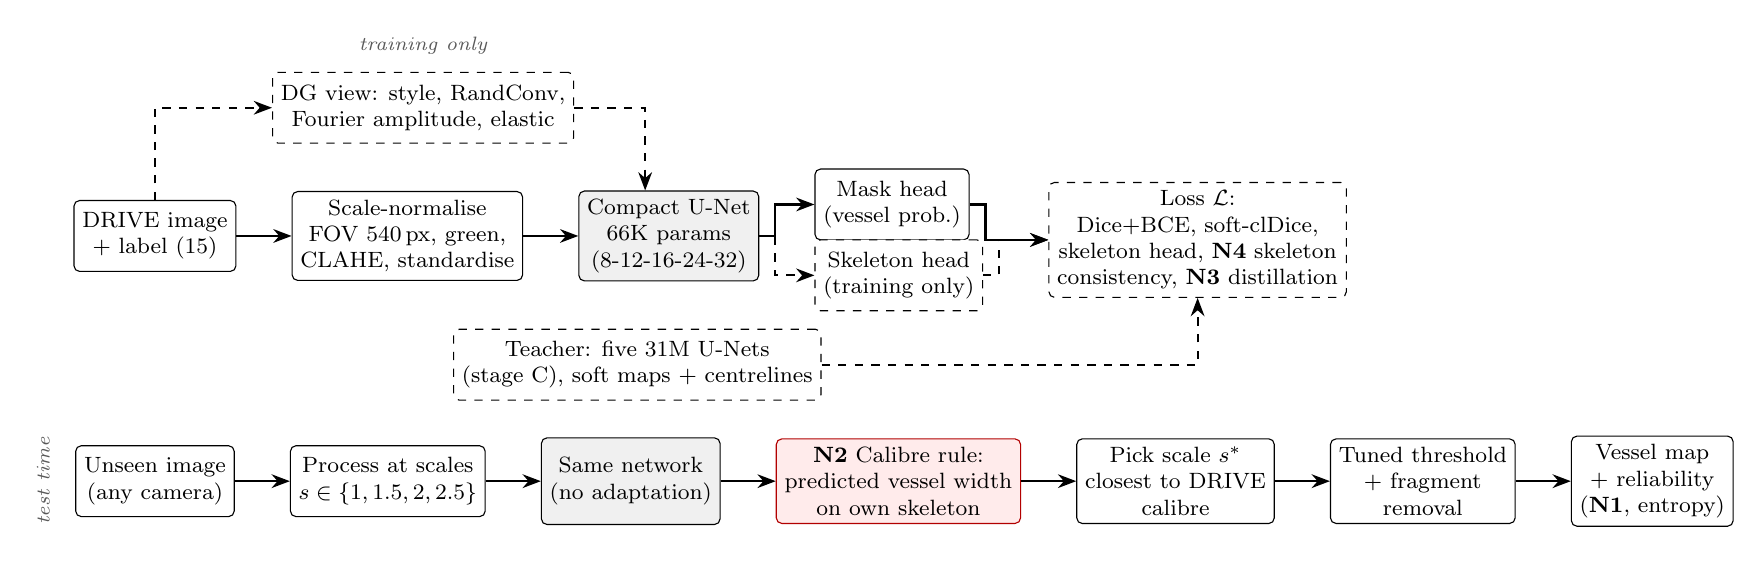
\begin{tikzpicture}[
  font=\footnotesize, >=Stealth,
  blk/.style={draw, rounded corners=2pt, align=center, minimum height=9mm, inner sep=3pt, fill=white},
  trn/.style={blk, dashed},
  net/.style={blk, fill=black!6, minimum height=11mm},
  hot/.style={blk, fill=red!8, draw=red!70!black},
  lab/.style={font=\scriptsize\itshape, text=black!65},
  arr/.style={->, thick},
  darr/.style={->, thick, dashed}
]
% ---------------------------------------------------------------- training row
\node[blk] (img) {DRIVE image\\+ label (15)};
\node[blk, right=7mm of img] (pre) {Scale-normalise\\FOV 540\,px, green,\\CLAHE, standardise};
\node[net, right=7mm of pre] (net) {Compact U-Net\\66K params\\(8-12-16-24-32)};
\node[blk, right=7mm of net, yshift=4mm] (mask) {Mask head\\(vessel prob.)};
\node[trn, right=7mm of net, yshift=-5mm] (skel) {Skeleton head\\(training only)};
\node[trn, right=8mm of mask, xshift=2mm, yshift=-4.5mm] (loss) {Loss $\mathcal L$:\\Dice+BCE, soft-clDice,\\skeleton head, \textbf{N4} skeleton\\consistency, \textbf{N3} distillation};
\node[trn, above=6mm of pre, xshift=2mm] (dg) {DG view: style, RandConv,\\Fourier amplitude, elastic};
\node[trn, below=6mm of net, xshift=-4mm] (teach) {Teacher: five 31M U-Nets\\(stage C), soft maps + centrelines};
\draw[arr] (img) -- (pre);
\draw[arr] (pre) -- (net);
\draw[arr] (net.east) -- ++(2mm,0) |- (mask.west);
\draw[darr] (net.east) -- ++(2mm,0) |- (skel.west);
\draw[arr] (mask.east) -- ++(2mm,0) |- (loss.west);
\draw[darr] (skel.east) -- ++(2mm,0) |- (loss.west);
\draw[darr] (img.north) |- (dg.west);
\draw[darr] (dg.east) -| ([xshift=-3mm]net.north);
\draw[darr] (teach.east) -| (loss.south);
\node[lab, above=1mm of dg] {training only};
% ---------------------------------------------------------------- test row
\node[blk, below=22mm of img] (timg) {Unseen image\\(any camera)};
\node[blk, right=7mm of timg] (scales) {Process at scales\\$s\in\{1,1.5,2,2.5\}$};
\node[net, right=7mm of scales] (net2) {Same network\\(no adaptation)};
\node[hot, right=7mm of net2] (cal) {\textbf{N2} Calibre rule:\\predicted vessel width\\on own skeleton};
\node[blk, right=7mm of cal] (sel) {Pick scale $s^{*}$\\closest to DRIVE\\calibre};
\node[blk, right=7mm of sel] (post) {Tuned threshold\\+ fragment\\removal};
\node[blk, right=7mm of post] (out) {Vessel map\\+ reliability\\(\textbf{N1}, entropy)};
\draw[arr] (timg) -- (scales);
\draw[arr] (scales) -- (net2);
\draw[arr] (net2) -- (cal);
\draw[arr] (cal) -- (sel);
\draw[arr] (sel) -- (post);
\draw[arr] (post) -- (out);
\node[lab, left=2mm of timg, rotate=90, anchor=south] {test time};
\end{tikzpicture}
}
\caption{TG-LiteNet v2.1. Training (top) uses a robustness-augmented second view, a skeleton head and a teacher; at test time (bottom) the same network is applied at several scales and the one whose predicted vessel calibre matches the training data is kept. Dashed boxes exist only during training; N1--N4 mark the new ideas.}
\label{fig:overview}
\end{figure*}

\subsection{Preprocessing and scale normalisation}
Cameras differ strongly in resolution (HRF images are $\sim$6$\times$ wider than DRIVE's), so the pixel width of vessels, to which convolutional networks are sensitive, changes with the dataset. Every image is rescaled so that its FOV is 540\,px wide (the median official DRIVE FOV width), which uses no label and no target statistic. We then keep the green channel, apply CLAHE~\cite{zuiderveld1994} (clip 2, 64-px tiles), and standardise inside the FOV. Predictions are resampled to the native resolution, and \emph{all metrics are computed inside the FOV against native-resolution labels}.

\subsection{Networks}
\textbf{Baseline} (stages A--C): the U-Net~\cite{ronneberger2015} with base width 64 (31.04\,M parameters, \gflopsA\ GFLOPs at $512^2$). \textbf{Compact backbone} (stages D--E): chosen \emph{before} any target evaluation among four candidates with at most 2\,M parameters, keeping those within 0.005 DRIVE-validation Dice of the best and taking the lowest CPU latency (Table~\ref{tab:backbone}); the rule selected a plain U-Net of width 8 (\compactParams K parameters, \gflopsE\ GFLOPs). \textbf{v2.1 network}: a U-Net with channels 8-12-16-24-32 (\hParamsExact\ parameters, 2.73 GFLOPs), chosen over a two-stage W-Net with 64K parameters (equal validation Dice, faster on CPU). Stage E adds spatial dropout ($p{=}0.1$) for MC-dropout uncertainty.

\begin{table}[t]
\centering
\caption{Compact-backbone selection (DRIVE validation only, 3 seeds, CPU: 4 threads, $512^2$). All candidates fall within the 0.005 tolerance; the fastest is chosen.}
\label{tab:backbone}
\footnotesize
\begin{tabular}{lrrrc}
\toprule
Candidate & Params & Val Dice & CPU ms & Chosen \\
\midrule
depthwise $w{=}16$ & 212K & 0.8163 & 109 &  \\
hybrid $w{=}16$ & 260K & 0.8172 & 89 &  \\
plain U-Net $w{=}8$ & 486K & 0.8162 & 39 & \checkmark \\
plain U-Net $w{=}16$ & 1942K & 0.8182 & 86 &  \\
\bottomrule
\end{tabular}
\end{table}

\subsection{Training objective}
With prediction $P$, label $G$, soft skeleton $S(\cdot)$ and FOV $F$, the total loss is
\begin{equation}
\mathcal L=\mathcal L_{\mathrm{Dice}}+\lambda_1\mathcal L_{\mathrm{BCE}}+\lambda_2\mathcal L_{\mathrm{clDice}}+\lambda_s\mathcal L_{\mathrm{skel}}+\lambda_3\mathcal L_{\mathrm{cons}},
\label{eq:loss}
\end{equation}
with $\lambda_1{=}1$ and $\lambda_2{=}\lambda_s{=}\lambda_3{=}0.5$ fixed in advance. Topology precision and sensitivity are $T_{\mathrm{prec}}=\sum S(P)\odot G/\sum S(P)$ and $T_{\mathrm{sens}}=\sum S(G)\odot P/\sum S(G)$, and $\mathcal L_{\mathrm{clDice}}=1-2T_{\mathrm{prec}}T_{\mathrm{sens}}/(T_{\mathrm{prec}}+T_{\mathrm{sens}})$. The skeleton head regresses the dilated skeleton of the label (Dice+BCE).

\textbf{Robustness augmentation.} From stage C on, each patch has a second view with illumination fields, blur, noise, JPEG artefacts and elastic deformation; v2.1 adds RandConv~\cite{xu2021randconv} and low-frequency Fourier amplitude jitter~\cite{xu2021fourier}, both computed from DRIVE images only. The consistency loss compares the two views. \textbf{N4} replaces the pixel form $\|\sigma(f(\tilde x))-\mathrm{sg}[\sigma(f(x))]\|^2$ by the skeleton form $1-\mathrm{softclDice}\big(P_{\mathrm{aug}},\mathrm{sg}[P_{\mathrm{clean}}]\big)$. \textbf{N3} adds, on the 15 training images, a distillation term~\cite{hinton2015} from a teacher made of the five 31M stage-C models: BCE between student and teacher probabilities, plus $\lambda_{kd}\,\mathrm{softclDice}(P_{\mathrm{student}},P_{\mathrm{teacher}})$ so that the student copies the teacher's soft \emph{centrelines}.

\subsection{Test-time scale selection (N2)}
HRF vessels are thin after FOV normalisation (Table~\ref{tab:data}), so a network trained at DRIVE's calibre sees unfamiliar widths. Algorithm~\ref{alg:scale} chooses the scale per image without labels or weight updates. The rule was set on DRIVE only: after a smoke test showed that the first candidate (lowest fragment density) is biased towards scale 1, it was replaced before any real run by calibre matching, which never moved off scale 1 on unmodified DRIVE-validation images and recovered most of the oracle gain on shrunken ones (Amendment 1 of the protocol).

\begin{algorithm}[t]
\caption{Calibre-guided scale selection}
\label{alg:scale}
\begin{algorithmic}[1]
\small
\REQUIRE image $I$, network $f$, scales $\mathcal S=\{1,1.5,2,2.5\}$, tuned threshold $\tau$, reference calibre $c^{*}$ (mean predicted calibre of $f$ on the 15 DRIVE training images)
\FOR{$s\in\mathcal S$}
  \STATE $P_s\leftarrow f(\mathrm{prep}(I\text{ at scale }s))$;\; $B_s\leftarrow[P_s\ge\tau]$
  \STATE $c_s\leftarrow$ mean of $2\,\mathrm{DT}(B_s)$ on the skeleton of $B_s$
\ENDFOR
\STATE $s^{*}\leftarrow\arg\min_{s}|c_s-c^{*}|$ (ties: smaller $s$)
\STATE resample $P_{s^{*}}$ to the normalised scale; apply $\tau$ and fragment removal
\end{algorithmic}
\end{algorithm}

\subsection{Reliability and uncertainty (N1, RQ4)}
Uncertainty is the binary entropy of the mean predicted probability for a single pass, for MC dropout ($T{=}20$) and for a five-model ensemble. The N1 score needs no extra passes: the number of 8-connected components per $10^5$ FOV pixels of the thresholded prediction (\texttt{rel\_frag}), with end-point density and small-fragment share as secondary scores.

% =============================================================================== V
\section{Experimental Setup}\label{sec:setup}
\subsection{Datasets and preprocessing}
Table~\ref{tab:data} lists the data. The prediction target is the binary vessel label of every pixel inside the field of view (FOV); the inputs are raw fundus photographs, so there are no missing values, categorical attributes or feature selection, and pre-processing is limited to the steps of Sec.~IV-A. DRIVE provides 20 training images, split once (seed 2026) into 15 for fitting and 5 for validation, and 20 test images (labels from the PaddleSeg mirror, checked against the official training labels). STARE (20), CHASE\_DB1 (28) and HRF (45) are used for testing only, and FIVES~\cite{jin2022fives} (200 test images) is reported separately and never averaged into ``unseen''. FOV masks are official for DRIVE and HRF and estimated for the others (checked visually). The vessel fraction is 9--13\% everywhere (class ratio about 1:8). The statistics quantify the shift: mean green intensity ranges from 53 (FIVES) to 109 (STARE), and the vessel calibre after FOV normalisation is about 3.5\,px except on HRF, where it is 1.4\,px because its labels are thin; HRF therefore also measures an annotation-style shift. \textbf{Availability:} DRIVE from \url{https://drive.grand-challenge.org} (test labels from the PaddleSeg mirror, SHA-256 pinned), STARE from \url{https://cecas.clemson.edu/~ahoover/stare}, CHASE\_DB1 from the Hugging Face mirror \texttt{MedOtter/CHASE\_DB1} (the Kingston server is offline), HRF from \url{https://www5.cs.fau.de/research/data/fundus-images} and FIVES from \url{https://doi.org/10.6084/m9.figshare.19688169}; checksums are recorded in \texttt{results/data/manifest.json} and no dataset is redistributed.

\begin{table}[t]
\centering
\caption{Datasets (statistics measured on the files used). Calibre: mean vessel width in pixels, native $\to$ after FOV normalisation; Green: mean$\pm$std inside the FOV.}
\label{tab:data}
\footnotesize
\setlength{\tabcolsep}{2.5pt}
\begin{adjustbox}{max width=\columnwidth}\begin{tabular}{lrcrrcccl}
\toprule
Dataset & \# & Size (px) & Vessel \% & FOV (px) & Calibre (px) & Green & FOV mask & Role \\
\midrule
DRIVE & 40 & 565$\times$584 & 12.6 & 540 & 3.5$\to$3.4 & 96$\pm$19 & official & train 15 / val 5 / test 20 \\
STARE & 20 & 700$\times$605 & 10.5 & 638 & 4.3$\to$3.5 & 109$\pm$24 & estimated & unseen test \\
CHASE\_DB1 & 28 & 999$\times$960 & 10.3 & 899 & 6.1$\to$3.6 & 62$\pm$26 & estimated & unseen test \\
HRF & 45 & 3504$\times$2336 & 9.1 & 3262 & 8.8$\to$1.4 & 60$\pm$17 & official & unseen test \\
FIVES & 200 & 2048$\times$2048 & 9.7 & 1969 & 13.2$\to$3.5 & 53$\pm$17 & estimated & extra test (200) \\
\bottomrule
\end{tabular}\end{adjustbox}
\end{table}

\subsection{Pre-registered protocol and training}
The rules of the study (data roles, pipeline, training, selection rules, metrics, comparisons) were written before any v2 model was trained; at the end of the DRIVE-only phases the suite recorded the SHA-256 of the protocol and configuration files and refused to evaluate any target before that (\texttt{protocol/decisions.json}); v2.1 has a second, hashed addendum. The targets are \emph{held-out, not untouched}: the v1 results of this project were known. All stages share one optimiser and schedule: AdamW~\cite{loshchilov2019} (learning rate $10^{-3}$, weight decay $10^{-4}$), 300 warm-up iterations then cosine decay, \budgetIters\ iterations of 16 patch views of $256^2$ px (16 clean patches, or 8 clean plus their 8 augmented views), gradient clipping 1, fp16 autocast, and the best checkpoint by DRIVE-validation Dice. Stages A--E use five seeds, controls and variants three. The suite (PyTorch~\cite{paszke2019} 2.11, CUDA 12.8; scikit-image~\cite{vanderwalt2014} for skeletons~\cite{zhang1984} and components) ran on one machine (RTX A4000 GPU, Core i9-12900K CPU); the exact package versions are in \texttt{requirements-lock.txt}.

\subsection{Reproducibility}
Every table, figure and number of this paper is generated by \texttt{scripts/make\_paper.py} from the committed per-image metrics of every model on every test image, each run's configuration, training curve, DRIVE-validation choices and cost, the hashed decision records and the full suite logs (\texttt{results/}); the trained weights (14\,GB) are not in the repository. The study is resumable (\texttt{scripts/run\_all.py}, \texttt{scripts/run\_v21.py}), unit-tested, and the instructions, dependencies and dataset requirements are in \texttt{README.md}.

\subsection{Evaluation modes, metrics and statistics}
Per model, three modes are chosen on DRIVE validation only: \emph{raw} (threshold 0.5, the headline), \emph{clean} (threshold 0.5 plus removal of 8-connected components smaller than $k$, chosen to minimise validation Betti-0 error) and \emph{tuned} (threshold maximising validation Dice, then $k$); v2.1 adds \emph{scale selection}. \textbf{Overlap:} Dice, precision, sensitivity. \textbf{Topology:} clDice with exact skeletons and Betti-0/Betti-1 errors, the absolute difference in the number of connected components ($\beta_0$, 8-connectivity) and loops ($\beta_1=\beta_0-\chi$). \textbf{Cost:} parameters, FLOPs, median latency (PyTorch CPU with 4 threads, ONNX Runtime, GPU) and, for the 66K model, INT8 size. \textbf{Uncertainty:} pixel-level and image-level Spearman $\rho$ against error, area under the risk--coverage curve (AURC, reported as the share of the random-to-oracle gap closed) and ECE~\cite{guo2017}. Comparisons are seed-paired mean differences with 95\% $t$-intervals, Holm-adjusted~\cite{holm1979} within pre-registered families, and image-level paired bootstraps~\cite{efron1979}; a difference is called \emph{clear} only if its interval excludes zero. ``Unseen'' is the equal-weight mean over STARE, CHASE\_DB1 and HRF, and $\pm$ is the standard deviation over seeds.

% =============================================================================== VI
\section{Experimental Results and Discussion}
\begin{table*}[t]
\centering
\caption{Staged ablation of study v2 (mean$\pm$std over 5 seeds; threshold 0.5 unless stated; unseen = STARE, CHASE\_DB1, HRF; CPU: 4 threads, one $512^2$ image).}
\label{tab:stages}
\small
\setlength{\tabcolsep}{4pt}
\begin{adjustbox}{max width=\textwidth}\begin{tabular}{l ccc c c c rr}
\toprule
Model & DRIVE Dice & Unseen Dice & Tuned Dice & clDice & Betti-0 & Gap & Params (M) & CPU (ms) \\
\midrule
A  U-Net & 0.825{\scriptsize$\pm$0.003} & 0.759{\scriptsize$\pm$0.007} & 0.762{\scriptsize$\pm$0.015} & 0.836{\scriptsize$\pm$0.003} & 72.8{\scriptsize$\pm$8.3} & 0.066{\scriptsize$\pm$0.009} & 31.04 & 936 \\
B  + topology loss & 0.821{\scriptsize$\pm$0.002} & 0.758{\scriptsize$\pm$0.004} & 0.775{\scriptsize$\pm$0.007} & 0.842{\scriptsize$\pm$0.007} & 33.9{\scriptsize$\pm$6.5} & 0.063{\scriptsize$\pm$0.004} & 31.04 & 989 \\
C  + DG augmentation & 0.824{\scriptsize$\pm$0.001} & 0.761{\scriptsize$\pm$0.004} & 0.789{\scriptsize$\pm$0.008} & 0.846{\scriptsize$\pm$0.002} & 35.5{\scriptsize$\pm$3.0} & 0.064{\scriptsize$\pm$0.003} & 31.04 & 1003 \\
D  compact backbone & 0.819{\scriptsize$\pm$0.001} & 0.749{\scriptsize$\pm$0.002} & 0.780{\scriptsize$\pm$0.002} & 0.835{\scriptsize$\pm$0.001} & 40.5{\scriptsize$\pm$3.8} & 0.070{\scriptsize$\pm$0.002} & 0.49 & 31 \\
E  TG-LiteNet & 0.817{\scriptsize$\pm$0.001} & 0.751{\scriptsize$\pm$0.006} & 0.780{\scriptsize$\pm$0.007} & 0.836{\scriptsize$\pm$0.002} & 39.2{\scriptsize$\pm$1.4} & 0.067{\scriptsize$\pm$0.007} & 0.49 & 30 \\
\midrule
E  + MC dropout ($T{=}20$) & 0.817{\scriptsize$\pm$0.002} & 0.752{\scriptsize$\pm$0.006} & 0.778{\scriptsize$\pm$0.007} & 0.836{\scriptsize$\pm$0.002} & 39.9{\scriptsize$\pm$1.5} & 0.066{\scriptsize$\pm$0.007} & 0.49 & 600 $\times$ 20 \\
\bottomrule
\end{tabular}\end{adjustbox}
\end{table*}

\begin{figure*}[t]
\centering
\safefig{0.86\textwidth}{fig_stages}
\caption{Stages A--E on each dataset (mean over seeds, whiskers: standard deviation). Betti-0 error is on a log scale; lower is better. FIVES is an additional target.}
\label{fig:stages}
\end{figure*}

\subsection{Staged ablation (RQ1--RQ3)}
Table~\ref{tab:stages} and Fig.~\ref{fig:stages} give the main comparison. \textbf{RQ1.} Topology supervision lowers the raw unseen Betti-0 error by \dABBetti\ ($\pm$\ciABBetti; Holm $p{=}\pABBetti$) and raises clDice by \dABCl\ ($\pm$\ciABCl), but changes Dice by only \dABDice\ ($\pm$\ciABDice); the Dice and clDice effects are not clear. \textbf{RQ2.} Adding the DG view changes unseen Dice by \dBCDice\ ($\pm$\ciBCDice, not clear) and the gap by \dBCGap; the strongest raw Dice comes from DG \emph{without} topology (\uDiceRawX\ against \uDiceRawA\ for the baseline, $\Delta=\dAXDice$, $\pm$\ciAXDice, secondary family), at the price of a raw Betti-0 error of \uBettiRawX. \textbf{RQ3.} Moving from 31M to \compactParams K parameters costs \dCDDice\ unseen Dice ($\pm$\ciCDDice) and \dCDCl\ clDice ($\pm$\ciCDCl, Holm $p{=}\pCDCl$), both clear; the gap widens by \dCDGap. In return the model is 64$\times$ smaller and 31$\times$ faster on CPU (\cpuE\ against \cpuA\,ms) and 8$\times$ faster on GPU. Dropout (D$\to$E) changes nothing measurable, and MC averaging adds \dMcDice\ ($\pm$\dMcDiceCi) Dice at 20$\times$ the cost.

\subsection{Fragments, threshold and the real cost of topology}
Fig.~\ref{fig:modes} repeats the finding of an earlier pilot with the pre-registered modes. \textbf{Clean:} deleting components below a validation-chosen size brings the unseen Betti-0 error of \emph{every} model to \uBettiCleanB--\uBettiCleanC\ (the U-Net falls from \uBettiRawA\ to \uBettiCleanA), with Dice changes of at most 0.003; raw fragment counts therefore do not measure topology. \textbf{Tuned:} the DRIVE-validation threshold raises unseen Dice to \uDiceTunedB\ (B), \uDiceTunedC\ (C), \uDiceTunedD\ (D) and \uDiceTunedE\ (E) but leaves the plain U-Net at \uDiceTunedA, and the tuned gap for C, D and E is \gapTunedC--\gapTunedD\ against \gapRawA\ at threshold 0.5. The Dice ``cost'' of topology at threshold 0.5 is thus largely calibration: topology-trained models over-segment at 0.5. Warming up the topology weight, as a pre-registered secondary test, changes unseen Dice by $+0.0023$ ($\pm0.0197$, not clear; tuned \uDiceTunedWarm\ against \uDiceTunedC).

\begin{figure}[t]
\centering
\safefig{0.86\columnwidth}{fig_modes}
\caption{Evaluation modes on the unseen datasets. (a) Raw and cleaned Betti-0 error; (b) Dice at threshold 0.5, after fragment removal, and with the validation-tuned threshold. U+DG: U-Net with DG augmentation and no topology loss.}
\label{fig:modes}
\end{figure}

\subsection{Discussion}
At threshold 0.5 every stage over-segments the unseen datasets: precision is only \precRawA--\precRawC\ against sensitivities of \sensRawA--\sensRawC, and the thresholds chosen on DRIVE validation are \thrA\ for the U-Net but \thrB--\thrE\ for the topology-trained models, which are more confident and so more over-segmenting. Raising the threshold lifts precision to \precTunedC\ (stage C) at a cost of about 0.04 sensitivity, which explains why the apparent Dice cost of topology supervision disappears. The remaining gap to DRIVE comes from HRF (unseen Dice 0.70--0.72 for stages A--E against 0.76--0.80 on STARE and CHASE\_DB1), where thin labels, large images and a different annotation style compound the camera shift; FIVES, whose vessels are thick and well contrasted, is the easiest target. These patterns are why a label-free adjustment of the processing scale helps on HRF and why it must not be applied blindly.

\subsection{Backbone and cost}
Depthwise-separable convolutions save parameters but not time: at DRIVE-validation parity, the 212K depthwise network needs \cpuKlite\,ms against \cpuKeight\,ms for the plain 486K U-Net and \cpuKsixteen\,ms for the plain 1.94\,M U-Net (Table~\ref{tab:backbone}). Depthwise layers perform little arithmetic per byte moved, so FLOP counts overstate their benefit on this CPU.

\subsection{Uncertainty (RQ4)}
\begin{table}[t]
\centering
\caption{Uncertainty on the unseen datasets (mean over STARE, CHASE\_DB1, HRF). $\rho_{px}$, $\rho_{img}$: Spearman correlation of uncertainty with pixel and image error; AURC gain: share of the random-to-oracle gap closed by rejecting the most uncertain images; ECE$_T$: after temperature scaling fitted on DRIVE validation.}
\label{tab:unc}
\footnotesize
\setlength{\tabcolsep}{3pt}
\begin{adjustbox}{max width=\columnwidth}\begin{tabular}{lccccc}
\toprule
Uncertainty source & $\rho_{px}$ & $\rho_{img}$ & AURC gain (\%) & ECE & ECE$_T$ \\
\midrule
A  U-Net (entropy) & 0.34 & -0.03 & -0.9 & 0.042 & 0.046 \\
C  + DG (entropy) & 0.34 & +0.01 & +1.7 & 0.045 & 0.052 \\
E  TG-LiteNet (entropy) & 0.34 & -0.08 & -9.9 & 0.046 & 0.053 \\
E  MC dropout ($T{=}20$) & 0.34 & -0.08 & -8.6 & 0.047 & 0.054 \\
D  5-model ensemble & 0.34 & -0.03 & +2.1 & 0.046 & 0.054 \\
\bottomrule
\end{tabular}\end{adjustbox}
\end{table}
Table~\ref{tab:unc} shows that entropy ranks erroneous \emph{pixels} moderately ($\rho_{px}\approx$ \rhoPxEmc) for every source, and rejecting the 10\% most uncertain pixels lowers the pixel error from \pxErrFull\% to \pxErrNinety\%. At image level, no source is reliably better than random: the correlation is negative on HRF (\rhoImgHrfE\ for a single pass, \rhoImgHrfEmc\ for MC dropout), and the AURC gains are small and unstable. Temperature scaling fitted on DRIVE validation does not transfer (ECE \eceE\ $\to$ \eceTsE). RQ4 is therefore supported for pixels and not for whole images, at 20$\times$ (MC dropout) or 5$\times$ (ensemble) the cost.

\subsection{The 66K model and test-time scale selection (v2.1)}
\begin{table*}[t]
\centering
\caption{v2.1 against v2 and published lightweight models (unseen datasets; tuned threshold unless stated; native-resolution scoring; Betti-0 is the raw error at threshold 0.5). Published numbers are context only: their training data, scoring resolution and thresholds differ. n/r: not reported.}
\label{tab:models}
\footnotesize
\setlength{\tabcolsep}{3pt}
\begin{adjustbox}{max width=\textwidth}\begin{tabular}{l rrr ccc cc c cc}
\toprule
Model & Params & GFLOPs & CPU ms & STARE & CHASE & HRF & Unseen & + scale sel. & FIVES & clDice & Betti-0 \\
\midrule
DSAE-Net~\cite{zeng2025} & 78K & 4.76 & -- & 0.819 & 0.815 & 0.801 & 0.812 & -- & -- & -- & -- \\
LightVesselNet~\cite{sobhan2026} & 75K & 1.4 & -- & -- & -- & -- & n/r & -- & -- & -- & -- \\
DGSSA~\cite{liu2026dgssa} (multi-source) & n/r & n/r & -- & -- & -- & -- & 0.780 & -- & -- & -- & -- \\
\midrule
v2 stage C (U-Net) & 31.0M & 384.74 & 1003 & 0.828{\scriptsize$\pm$0.005} & 0.789{\scriptsize$\pm$0.006} & 0.749{\scriptsize$\pm$0.013} & 0.789{\scriptsize$\pm$0.008} & 0.751{\scriptsize$\pm$0.034} & 0.842{\scriptsize$\pm$0.008} & 0.836{\scriptsize$\pm$0.003} & 35.5{\scriptsize$\pm$3.0} \\
\midrule
v2 stage E (TG-LiteNet) & 486K & 6.05 & 30 & 0.819{\scriptsize$\pm$0.003} & 0.787{\scriptsize$\pm$0.004} & 0.733{\scriptsize$\pm$0.014} & 0.780{\scriptsize$\pm$0.007} & 0.789{\scriptsize$\pm$0.005} & 0.847{\scriptsize$\pm$0.006} & 0.825{\scriptsize$\pm$0.003} & 39.2{\scriptsize$\pm$1.5} \\
v2.1 compact U-Net & 486K & 6.05 & 55 & 0.812{\scriptsize$\pm$0.004} & 0.775{\scriptsize$\pm$0.011} & 0.736{\scriptsize$\pm$0.016} & 0.775{\scriptsize$\pm$0.010} & 0.785{\scriptsize$\pm$0.009} & 0.822{\scriptsize$\pm$0.007} & 0.826{\scriptsize$\pm$0.004} & 31.8{\scriptsize$\pm$6.9} \\
v2.1 depthwise (size-rule headline) & 212K & 5.53 & 107 & 0.812{\scriptsize$\pm$0.007} & 0.777{\scriptsize$\pm$0.009} & 0.736{\scriptsize$\pm$0.017} & 0.775{\scriptsize$\pm$0.011} & 0.785{\scriptsize$\pm$0.008} & 0.822{\scriptsize$\pm$0.007} & 0.826{\scriptsize$\pm$0.000} & 29.0{\scriptsize$\pm$3.4} \\
\textbf{v2.1 TG-LiteNet 66K} & 66K & 2.73 & 25 & 0.810{\scriptsize$\pm$0.002} & 0.765{\scriptsize$\pm$0.006} & 0.729{\scriptsize$\pm$0.005} & 0.768{\scriptsize$\pm$0.004} & 0.779{\scriptsize$\pm$0.004} & 0.810{\scriptsize$\pm$0.013} & 0.820{\scriptsize$\pm$0.003} & 32.1{\scriptsize$\pm$2.2} \\
v2.1 66K, 5-model ensemble & 66K & 2.73 & 25 & 0.817 & 0.772 & 0.730 & 0.773 & 0.785 & 0.828 & 0.827 & 26.5 \\
\bottomrule
\end{tabular}\end{adjustbox}
\end{table*}

\begin{figure*}[t]
\centering
\safefig{0.86\textwidth}{fig_cost_scale}
\caption{(a, b) Unseen Dice against size and CPU time (v2 grey/orange, v2.1 blue/red; the star is a published number under a different protocol). (c) Change in Dice from calibre-guided scale selection, by dataset.}
\label{fig:cost}
\end{figure*}

Table~\ref{tab:models} and Fig.~\ref{fig:cost} summarise v2.1. The \hParamsK K model is \ratioParams$\times$ smaller than the U-Net and 7.4$\times$ smaller than the v2 model, needs 2.73 GFLOPs and \HCpu\,ms per image, and reaches \HTuned\ unseen Dice with a tuned threshold (\HRaw\ at 0.5) against \CvTuned\ for the 31M U-Net, with a raw Betti-0 error of \HBetti. It is \hFpKb\,KB as FP32 and \hIntKb\,KB as static INT8 with unchanged Dice on all five datasets, although INT8 was slower on this CPU (\hFpMs\ against \hIntMs\,ms). \textbf{Disclosure:} the pre-registered size rule (smallest model within 0.005 validation Dice of the best) selected the 212K depthwise network as the formal headline, because the 66K model trailed it by \valGap; we therefore show the 66K model as the efficiency point and report both.

\textbf{Scale selection (N2).} Calibre-guided selection raises the unseen Dice of the 66K model by \nTwoH\ ($\pm$\nTwoHci, clear), by \nTwoRl\ and \nTwoRu\ for the two reference networks and by \nTwoEv\ for v2 stage E (all clear). The gain comes from HRF (\nTwoHrf\ for the 66K model, where the rule picks scale 1.5 for \scaleOneFiveHrf\% of images) and is zero on STARE and CHASE\_DB1, where it keeps scale 1. It is best suited to thin vessels: on FIVES (\nTwoFives) and on the 31M stage-C model (\nTwoCv, clear) the default scale is the better choice, so a thick-vessel guard is a natural refinement; the rule passed its DRIVE-validation safety check for every model. Fig.~\ref{fig:mech} shows why: HRF vessels are predicted thinner than DRIVE's at scale 1 and match them at scale 1.5, whereas the other datasets already match.

\begin{figure}[t]
\centering
\safefig{0.88\columnwidth}{fig_scale_mech}
\caption{Mechanism of calibre-guided scale selection for the 66K model. (a) Mean predicted vessel width at each input scale, per dataset. (b) Share of images assigned to each scale.}
\label{fig:mech}
\end{figure}

\begin{table}[t]
\centering
\caption{Pixel-level classification metrics of the 66K model (tuned threshold, native resolution, mean over images and 5 seeds). F1 equals the per-image Dice. TP/FP/FN/TN: confusion matrix in \% of field-of-view pixels.}
\label{tab:conf}
\footnotesize
\setlength{\tabcolsep}{2.6pt}
\begin{adjustbox}{max width=\columnwidth}\begin{tabular}{l ccccc cccc}
\toprule
Dataset & Acc & Prec & Rec & Spec & F1 & TP & FP & FN & TN \\
\midrule
STARE & 0.958 & 0.766 & 0.864 & 0.969 & 0.810 & 9.1 & 2.8 & 1.4 & 86.8 \\
CHASE & 0.945 & 0.676 & 0.882 & 0.952 & 0.765 & 9.1 & 4.3 & 1.2 & 85.4 \\
HRF & 0.946 & 0.666 & 0.814 & 0.960 & 0.729 & 7.4 & 3.7 & 1.7 & 87.2 \\
\midrule
FIVES & 0.966 & 0.806 & 0.825 & 0.979 & 0.810 & 8.2 & 1.9 & 1.5 & 88.4 \\
\bottomrule
\end{tabular}\end{adjustbox}
\end{table}

\textbf{Pixel-level classification metrics.} Vessel segmentation is a binary classification of every pixel in the field of view, so Table~\ref{tab:conf} gives accuracy, precision, recall, specificity, F1 and the confusion matrix. Accuracy is high on every dataset but is dominated by the background (\confTnLo--\confTnHi\% of pixels are true negatives), which is why Dice (= F1) is our headline. On STARE, CHASE\_DB1 and HRF recall exceeds precision: the tuned threshold favours sensitivity, so the remaining error is mostly over-segmentation (false positives \confFpLo--\confFpHi\% of pixels against \confFnLo--\confFnHi\% false negatives).

\textbf{Against published work.} The 66K model is within 0.01 of DSAE-Net on STARE but about 0.05 below on CHASE\_DB1 and 0.07 on HRF (\HChase\ and \HHrf\ against 0.815 and 0.801 published). The same gap appears for the 31M U-Net, so it stems from single-dataset training and native-resolution scoring, not from model size.

\begin{figure*}[t]
\centering
\safefig{0.66\textwidth}{fig_qualitative}
\caption{Example predictions, in the normalised-scale space the networks operate in (black: correct vessel, red: false positive, blue: missed). HRF (top) benefits from scale selection; on FIVES (bottom) the default scale is the better choice. Dice values are per image.}
\label{fig:qual}
\end{figure*}

\subsection{Novelties N1--N4}
\begin{table}[t]
\centering
\caption{Pre-registered verdicts for the four v2.1 novelties (3 seeds for ablations, so a result that is not yet clear is \emph{open}, not \emph{no effect}).}
\label{tab:novel}
\footnotesize
\setlength{\tabcolsep}{3pt}
\begin{adjustbox}{max width=\columnwidth}\begin{tabular}{l p{4.5cm} p{1.5cm}}
\toprule
 & Novelty and result (66K model, unseen, tuned) & Verdict \\
\midrule
N1 & Connectivity reliability score. $\rho$(fragments) $-$ $\rho$(entropy): $+0.1073$ against MC dropout (stage E), $\ensuremath{-}0.1374$ for the 66K model & Not met \\
N2 & Calibre-guided scale selection. Unseen Dice $+0.0114\,[\pm0.0005]$ (66K); HRF $+0.034$, FIVES $\ensuremath{-}0.061$ & \textbf{Supported} \\
N3 & Topology-aware distillation. $\Delta$Dice $\ensuremath{-}0.0051\,[\pm0.0148]$, $\Delta$clDice $+0.0019$ & Not shown \\
N4 & Skeleton-level consistency. $\Delta$Dice $\ensuremath{-}0.0091\,[\pm0.0045]$ (clear), $\Delta$clDice $+0.0011$ & Harms Dice \\
-- & RandConv + Fourier augmentation. $\Delta$Dice $\ensuremath{-}0.0094\,[\pm0.0267]$ & Not shown \\
\bottomrule
\end{tabular}\end{adjustbox}
\end{table}
Table~\ref{tab:novel} lists the outcomes. \textbf{N1}: the fragment-density score beat MC-dropout entropy for stage E (\nOneVsMc, $\pm$\nOneVsMcci) but not single-pass entropy (\nOneEd, not clear), and entropy was the stronger score for the 66K model (\nOneH); two secondary connectivity scores (end-point density, small-fragment share) ranked failures better than entropy for most models ($\rho\approx$ 0.2--0.3 against 0.0--0.2), a promising lead for follow-up. \textbf{N3} (centreline distillation) and the new augmentation show no clear effect yet, and \textbf{N4} trades Dice (\aNfourDice) for no clear connectivity benefit, so pixel-level consistency stays the recommended choice. The topology loss and skeleton head inherited from v2 keep the 66K maps well connected.

% =============================================================================== VII
\section{Ablation Analysis}
\begin{table}[t]
\centering
\caption{Full 2$\times$2$\times$2 factorial (backbone $\times$ topology loss $\times$ DG augmentation), unseen datasets, threshold 0.5 unless stated.}
\label{tab:factorial}
\footnotesize
\setlength{\tabcolsep}{3pt}
\begin{adjustbox}{max width=\columnwidth}\begin{tabular}{lcc c cccc c}
\toprule
Backbone & Topo & DG & n & Dice & clDice & Betti-0 & Tuned Dice & Tuned gap \\
\midrule
U-Net & -- & -- & 5 & 0.759{\scriptsize$\pm$0.007} & 0.836{\scriptsize$\pm$0.003} & 72.8{\scriptsize$\pm$8.3} & 0.762{\scriptsize$\pm$0.015} & 0.061{\scriptsize$\pm$0.014} \\
U-Net & -- & \checkmark & 3 & 0.774{\scriptsize$\pm$0.006} & 0.838{\scriptsize$\pm$0.001} & 91.1{\scriptsize$\pm$13.7} & 0.785{\scriptsize$\pm$0.007} & 0.042{\scriptsize$\pm$0.007} \\
U-Net & \checkmark & -- & 5 & 0.758{\scriptsize$\pm$0.004} & 0.842{\scriptsize$\pm$0.007} & 33.9{\scriptsize$\pm$6.5} & 0.775{\scriptsize$\pm$0.007} & 0.043{\scriptsize$\pm$0.006} \\
U-Net & \checkmark & \checkmark & 5 & 0.761{\scriptsize$\pm$0.004} & 0.846{\scriptsize$\pm$0.002} & 35.5{\scriptsize$\pm$3.0} & 0.789{\scriptsize$\pm$0.008} & 0.035{\scriptsize$\pm$0.009} \\
\midrule
Compact & -- & -- & 3 & 0.754{\scriptsize$\pm$0.003} & 0.825{\scriptsize$\pm$0.004} & 98.8{\scriptsize$\pm$13.5} & 0.753{\scriptsize$\pm$0.010} & 0.065{\scriptsize$\pm$0.011} \\
Compact & -- & \checkmark & 3 & 0.760{\scriptsize$\pm$0.001} & 0.827{\scriptsize$\pm$0.003} & 89.0{\scriptsize$\pm$2.6} & 0.773{\scriptsize$\pm$0.003} & 0.046{\scriptsize$\pm$0.005} \\
Compact & \checkmark & -- & 3 & 0.747{\scriptsize$\pm$0.005} & 0.835{\scriptsize$\pm$0.001} & 44.5{\scriptsize$\pm$5.4} & 0.762{\scriptsize$\pm$0.005} & 0.052{\scriptsize$\pm$0.006} \\
Compact & \checkmark & \checkmark & 5 & 0.749{\scriptsize$\pm$0.002} & 0.835{\scriptsize$\pm$0.001} & 40.5{\scriptsize$\pm$3.8} & 0.780{\scriptsize$\pm$0.002} & 0.039{\scriptsize$\pm$0.002} \\
\bottomrule
\end{tabular}\end{adjustbox}
\end{table}
Table~\ref{tab:factorial} separates the factors. \emph{Topology loss} lowers the raw Betti-0 error in all four pairs and raises clDice by 0.006--0.010, but lowers raw Dice when DG is present (\dXCDice\ $\pm$\ciXCDice, clDice \dXCCl). \emph{DG augmentation} adds 0.006--0.015 raw Dice without topology supervision (U-Net: \dAXDice, $\pm$\ciAXDice) and only 0.002--0.003 with it. The \emph{compact backbone} costs Dice and clDice in every pair (tuned Dice \uDiceTunedC\ against \uDiceTunedD\ for stages C and D). The cbDice and Skeleton Recall variants match soft-clDice at best (unseen Dice 0.736 and 0.726 at 0.5), and removing the skeleton head or the consistency loss changes unseen Dice by less than 0.002. Accuracy saturates at width 16 (tuned Dice 0.786 at $w{=}16$ and $w{=}24$, 0.785 at $w{=}32$, 0.779 at $w{=}8$).

% =============================================================================== VIII
\section{Conclusion and Future Work}
\textbf{Findings.} Under a pre-registered, single-dataset protocol, soft-clDice with a skeleton head reduces raw fragment counts but not more than a simple clean-up step, and its Dice cost is a threshold-calibration effect. Robustness augmentation helps without topology supervision. A plain compact U-Net is 31$\times$ faster than a 31M U-Net for $\approx$0.01 Dice, and depthwise convolutions are not faster. A \hParamsK K-parameter model reaches \HTuned\ (\HSel\ with calibre-guided scale selection) unseen Dice, 3--4 points below the best published lightweight network evaluated under different protocols. Of four new topology-based ideas, test-time scale selection is clearly supported, the connectivity reliability score yields a promising lead, and distillation and skeleton consistency define what to test next with more seeds and data. \textbf{Objectives.} O1 and O2 were met (\nTrainAll\ trained models, rules fixed before evaluation); O3 was met in size, not in accuracy parity.
\textbf{Limitations.} (i) Fifteen training images and a single training dataset; (ii) three seeds for ablations give low power, and the ensembles are single instances; (iii) FOV masks are estimated for three datasets and labels come from one observer; (iv) the targets were seen in v1 and are held-out, not untouched; (v) the pre-registered size rule selected the 212K model as the formal headline, and scale selection is best suited to thin-vessel data; (vi) latencies come from one machine and INT8 was slower than FP32 on it; (vii) published numbers are context only. \textbf{Future work:} multi-dataset or patient-split training, a safeguard that disables scale selection on thick-vessel data, topology metrics robust to fragments, and INT8 measurements on an edge CPU. The code, protocol, per-run records and an interactive project page are public at \url{https://github.com/Deltasthicc/ML-Project}.

\section*{Acknowledgment}
The authors thank the CSD361 teaching staff for the project guidelines and feedback. \textbf{Author contributions.} The work is split by the three parts of the name TG-LiteNet. A.~Agarwal (Topology): topology losses and metrics, uncertainty and calibration, statistics, N1. T.~Shitanshu (Generalisation): data pipeline, augmentation and consistency, pre-registered protocol, N2, N4. S.~Rajan (Lite): backbones and model selection, distillation (N3), cost and INT8 measurement, training system.

\begin{thebibliography}{99}
\bibitem{liu2025review} Z. Liu, M. S. Sunar, T. S. Tan, and W. H. Wan Hitam, ``Deep learning for retinal vessel segmentation: a systematic review of techniques and applications,'' \emph{Med. Biol. Eng. Comput.}, vol. 63, no. 8, pp. 2191--2208, 2025.
\bibitem{ronneberger2015} O. Ronneberger, P. Fischer, and T. Brox, ``U-Net: Convolutional networks for biomedical image segmentation,'' in \emph{Proc. MICCAI}, 2015, pp. 234--241.
\bibitem{staal2004} J. Staal, M. D. Abr\`amoff, M. Niemeijer, M. A. Viergever, and B. van Ginneken, ``Ridge-based vessel segmentation in color images of the retina,'' \emph{IEEE Trans. Med. Imag.}, vol. 23, no. 4, pp. 501--509, 2004.
\bibitem{hoover2000} A. Hoover, V. Kouznetsova, and M. Goldbaum, ``Locating blood vessels in retinal images by piecewise threshold probing of a matched filter response,'' \emph{IEEE Trans. Med. Imag.}, vol. 19, no. 3, pp. 203--210, 2000.
\bibitem{fraz2012} M. M. Fraz \emph{et al.}, ``An ensemble classification-based approach applied to retinal blood vessel segmentation,'' \emph{IEEE Trans. Biomed. Eng.}, vol. 59, no. 9, pp. 2538--2548, 2012.
\bibitem{budai2013} A. Budai, R. Bock, A. Maier, J. Hornegger, and G. Michelson, ``Robust vessel segmentation in fundus images,'' \emph{Int. J. Biomed. Imaging}, vol. 2013, 2013.
\bibitem{shit2021} S. Shit \emph{et al.}, ``clDice --- a novel topology-preserving loss function for tubular structure segmentation,'' in \emph{Proc. IEEE/CVF CVPR}, 2021, pp. 16\,560--16\,569.
\bibitem{shi2024} P. Shi, J. Hu, Y. Yang, Z. Gao, W. Liu, and T. Ma, ``Centerline boundary Dice loss for vascular segmentation,'' in \emph{Proc. MICCAI}, LNCS 15008, 2024, pp. 46--56.
\bibitem{kirchhoff2024} Y. Kirchhoff \emph{et al.}, ``Skeleton recall loss for connectivity conserving and resource efficient segmentation of thin tubular structures,'' in \emph{Proc. ECCV}, LNCS 15135, 2024, pp. 218--234.
\bibitem{hu2019} X. Hu, F. Li, D. Samaras, and C. Chen, ``Topology-preserving deep image segmentation,'' in \emph{Proc. NeurIPS}, 2019.
\bibitem{huang2026} Y. Huang, T. Miyazaki, K. Xu, X. Liu, Y. Fan, and S. Omachi, ``Topology-aware parameter-efficient adaptation for cross-dataset retinal vessel segmentation,'' arXiv:2609.26189, 2026.
\bibitem{galdran2022} A. Galdran \emph{et al.}, ``State-of-the-art retinal vessel segmentation with minimalistic models,'' \emph{Sci. Rep.}, vol. 12, art. 6174, 2022.
\bibitem{fadugba2024} J. Fadugba, P. K\"ohler, L. Koch, P. Manescu, and P. Berens, ``Benchmarking retinal blood vessel segmentation models for cross-dataset and cross-disease generalization,'' arXiv:2406.14994, 2024.
\bibitem{sobhan2026} S. Sobhan and F. Jalil, ``LightVesselNet: An ultra-lightweight sub-100K parameter network for retinal blood vessel segmentation,'' arXiv:2606.05354, 2026.
\bibitem{liu2026dgssa} B. Liu, Y. Zhang, S. Wang, S. Li, and J. Hong, ``DGSSA: Domain generalization with structural and stylistic augmentation for retinal vessel segmentation,'' \emph{Neural Netw.}, vol. 194, art. 108118, 2026.
\bibitem{wang2026wavernet} C. Wang, Y. Wang, Q. Xu, and G. Chen, ``WaveRNet: Wavelet-guided frequency learning for multi-source domain-generalized retinal vessel segmentation,'' arXiv:2601.05942, 2026.
\bibitem{hu2024hessian} D. Hu, H. Li, H. Liu, and I. Oguz, ``Domain generalization for retinal vessel segmentation via Hessian-based vector field,'' \emph{Med. Image Anal.}, vol. 95, art. 103164, 2024.
\bibitem{liu2025graphseg} K. Liu, S. Gao, Y. Fu, and S. Gao, ``Towards generalizable retina vessel segmentation with deformable graph priors,'' in \emph{Proc. NeurIPS}, 2025.
\bibitem{zeng2025} Z. Zeng, J. Liu, X. Huang, K. Luo, X. Yuan, and Y. Zhu, ``Efficient retinal vessel segmentation with 78K parameters,'' \emph{J. Imaging}, vol. 11, no. 9, art. 306, 2025.
\bibitem{ahmed2026} I. Ahmed, S. Absar, A. A. Sami, S. Sakib, D. Biswas, and S. A. M. Mostafa, ``TFFM: Topology-aware feature fusion module via latent graph reasoning for retinal vessel segmentation,'' arXiv:2601.19136, 2026.
\bibitem{zhou2025} J. Zhou \emph{et al.}, ``TopoTTA: Topology-enhanced test-time adaptation for tubular structure segmentation,'' in \emph{Proc. IEEE/CVF ICCV}, 2025, pp. 24\,123--24\,134.
\bibitem{khazem2026} S. Khazem, ``TopoLoRA-SAM: Topology-aware parameter-efficient adaptation of foundation segmenters for thin-structure and cross-domain binary semantic segmentation,'' arXiv:2601.02273, 2026.
\bibitem{gupta2023} S. Gupta, Y. Zhang, X. Hu, P. Prasanna, and C. Chen, ``Topology-aware uncertainty for image segmentation,'' in \emph{Proc. NeurIPS}, 2023.
\bibitem{gal2016} Y. Gal and Z. Ghahramani, ``Dropout as a Bayesian approximation: Representing model uncertainty in deep learning,'' in \emph{Proc. ICML}, 2016, pp. 1050--1059.
\bibitem{ovadia2019} Y. Ovadia \emph{et al.}, ``Can you trust your model's uncertainty? Evaluating predictive uncertainty under dataset shift,'' in \emph{Proc. NeurIPS}, 2019.
\bibitem{zuiderveld1994} K. Zuiderveld, ``Contrast limited adaptive histogram equalization,'' in \emph{Graphics Gems IV}. Academic Press, 1994, pp. 474--485.
\bibitem{howard2017} A. G. Howard \emph{et al.}, ``MobileNets: Efficient convolutional neural networks for mobile vision applications,'' arXiv:1704.04861, 2017.
\bibitem{paszke2019} A. Paszke \emph{et al.}, ``PyTorch: An imperative style, high-performance deep learning library,'' in \emph{Proc. NeurIPS}, 2019.
\bibitem{vanderwalt2014} S. van der Walt \emph{et al.}, ``scikit-image: image processing in Python,'' \emph{PeerJ}, vol. 2, art. e453, 2014.
\bibitem{zhang1984} T. Y. Zhang and C. Y. Suen, ``A fast parallel algorithm for thinning digital patterns,'' \emph{Commun. ACM}, vol. 27, no. 3, pp. 236--239, 1984.
\bibitem{xu2021randconv} Z. Xu, D. Liu, J. Yang, C. Raffel, and M. Niethammer, ``Robust and generalizable visual representation learning via random convolutions,'' in \emph{Proc. ICLR}, 2021.
\bibitem{xu2021fourier} Q. Xu, R. Zhang, Y. Zhang, Y. Wang, and Q. Tian, ``A Fourier-based framework for domain generalization,'' in \emph{Proc. IEEE/CVF CVPR}, 2021, pp. 14\,383--14\,392.
\bibitem{hinton2015} G. Hinton, O. Vinyals, and J. Dean, ``Distilling the knowledge in a neural network,'' arXiv:1503.02531, 2015.
\bibitem{lakshminarayanan2017} B. Lakshminarayanan, A. Pritzel, and C. Blundell, ``Simple and scalable predictive uncertainty estimation using deep ensembles,'' in \emph{Proc. NeurIPS}, 2017, pp. 6402--6413.
\bibitem{guo2017} C. Guo, G. Pleiss, Y. Sun, and K. Q. Weinberger, ``On calibration of modern neural networks,'' in \emph{Proc. ICML}, 2017, pp. 1321--1330.
\bibitem{loshchilov2019} I. Loshchilov and F. Hutter, ``Decoupled weight decay regularization,'' in \emph{Proc. ICLR}, 2019.
\bibitem{holm1979} S. Holm, ``A simple sequentially rejective multiple test procedure,'' \emph{Scand. J. Statist.}, vol. 6, no. 2, pp. 65--70, 1979.
\bibitem{efron1979} B. Efron, ``Bootstrap methods: another look at the jackknife,'' \emph{Ann. Statist.}, vol. 7, no. 1, pp. 1--26, 1979.
\bibitem{jin2022fives} K. Jin \emph{et al.}, ``FIVES: A fundus image dataset for artificial intelligence based vessel segmentation,'' \emph{Sci. Data}, vol. 9, art. 475, 2022.
\end{thebibliography}
\end{document}
